\documentclass[12pt]{article}

\usepackage{hcmus-report-template}
\usepackage{longtable}
\usepackage{enumitem}
\usepackage{tikz}
\usetikzlibrary{arrows.meta, positioning, shapes.geometric}

% Disable indentation on new paragraphs
\setlength{\parindent}{0pt}

% Line spacing 1.5
\renewcommand{\baselinestretch}{1.5}

% Graphic path
\graphicspath{{img/}}

% Define course name, report name and report title.
\newcommand{\coursename}{CS426 --- Mobile Device Application Development}
\newcommand{\reportname}{The Code Cup}
\newcommand{\reporttitle}{Midterm Project Report}

\newcommand{\studentname}{Trinh Vo Nam Kiet (24125013)}
\newcommand{\teachername}{} % Fill in if applicable

% Header
\lhead{\reporttitle}
\rhead{
University of Science {--} VNUHCM\\
\coursename{}
}

% Footer
\newcommand{\leftfooter}{The Code Cup --- CS426 Midterm}
\lfoot{\leftfooter}

% ============ DOCUMENT ============
\begin{document}

\pagenumbering{roman}
\begin{titlepage}
    \newcommand{\HRule}{\rule{\linewidth}{0.5mm}}
    \centering

    \textsc{\LARGE Vietnam National University HCMC}\\[0.5cm]
    \textsc{\Large University of Science}\\[0.5cm]
    \textsc{\large Faculty of Information Technology}\\[0.5cm]

    \HRule{}\\[0.4cm]
    {
    \huge{\bfseries{\reporttitle}}\\[0.5cm]
    \large{\bfseries{\reportname}}
    }\\[0.4cm]
    \HRule{}\\[0.5cm]

    \textbf{\large Course: \coursename}\\[0.5cm]

    \begin{minipage}[t]{0.4\textwidth}
        \begin{flushleft} \large
            \emph{Student:}\\
            \studentname{}
        \end{flushleft}
    \end{minipage}
    {~}
    \begin{minipage}[t]{0.4\textwidth}
        \begin{flushright} \large
            \emph{Instructor:} \\
            \teachername{}
        \end{flushright}
    \end{minipage}\\[1cm]

    {\large \today}\\[1cm]

    \includegraphics[scale=.20]{hcmus-logo.png}\\[1cm]

    \vfill
\end{titlepage}


\tableofcontents
\pagebreak
\listoftables
\pagebreak
\listoffigures
\pagebreak

\pagenumbering{arabic}
\setcounter{page}{1}

\section{Introduction}

\textbf{The Code Cup} is a mobile coffee shop application built with Flutter, targeting Android. Users can browse a coffee menu, customize and order drinks, collect loyalty stamps, earn and redeem reward points, and manage their profile.

\subsection{Technology Stack}

\begin{itemize}
  \item \textbf{Framework:} Flutter (Dart)
  \item \textbf{Target platform:} Android
  \item \textbf{Architecture:} MVVM (Model--View--ViewModel)
  \item \textbf{State management:} \texttt{ChangeNotifier}
  \item \textbf{Persistence:} \texttt{SharedPreferences}
  \item \textbf{Testing:} \texttt{flutter\_test} (unit + widget tests)
\end{itemize}

\subsection{Codebase Statistics}

\begin{table}[H]
\centering
\caption{Codebase metrics}
\begin{tabular}{lr}
  \toprule
  Metric & Count \\
  \midrule
  Source files (\texttt{lib/}) & 34 \\
  Source lines of code & 3{,}824 \\
  Test files (\texttt{tests/}) & 18 \\
  Test lines of code & 1{,}952 \\
  Total tests & 144 \\
  \quad Unit tests & 89 \\
  \quad UI (widget) tests & 55 \\
  Pass rate & 100\% \\
  \bottomrule
\end{tabular}
\end{table}

% ══════════════════════════════════════════════════════════
\section{Architecture}

The application follows the \textbf{Model--View--ViewModel (MVVM)} pattern with manual dependency injection (no DI framework).

\subsection{Layer Diagram}

\begin{figure}[H]
  \centering
  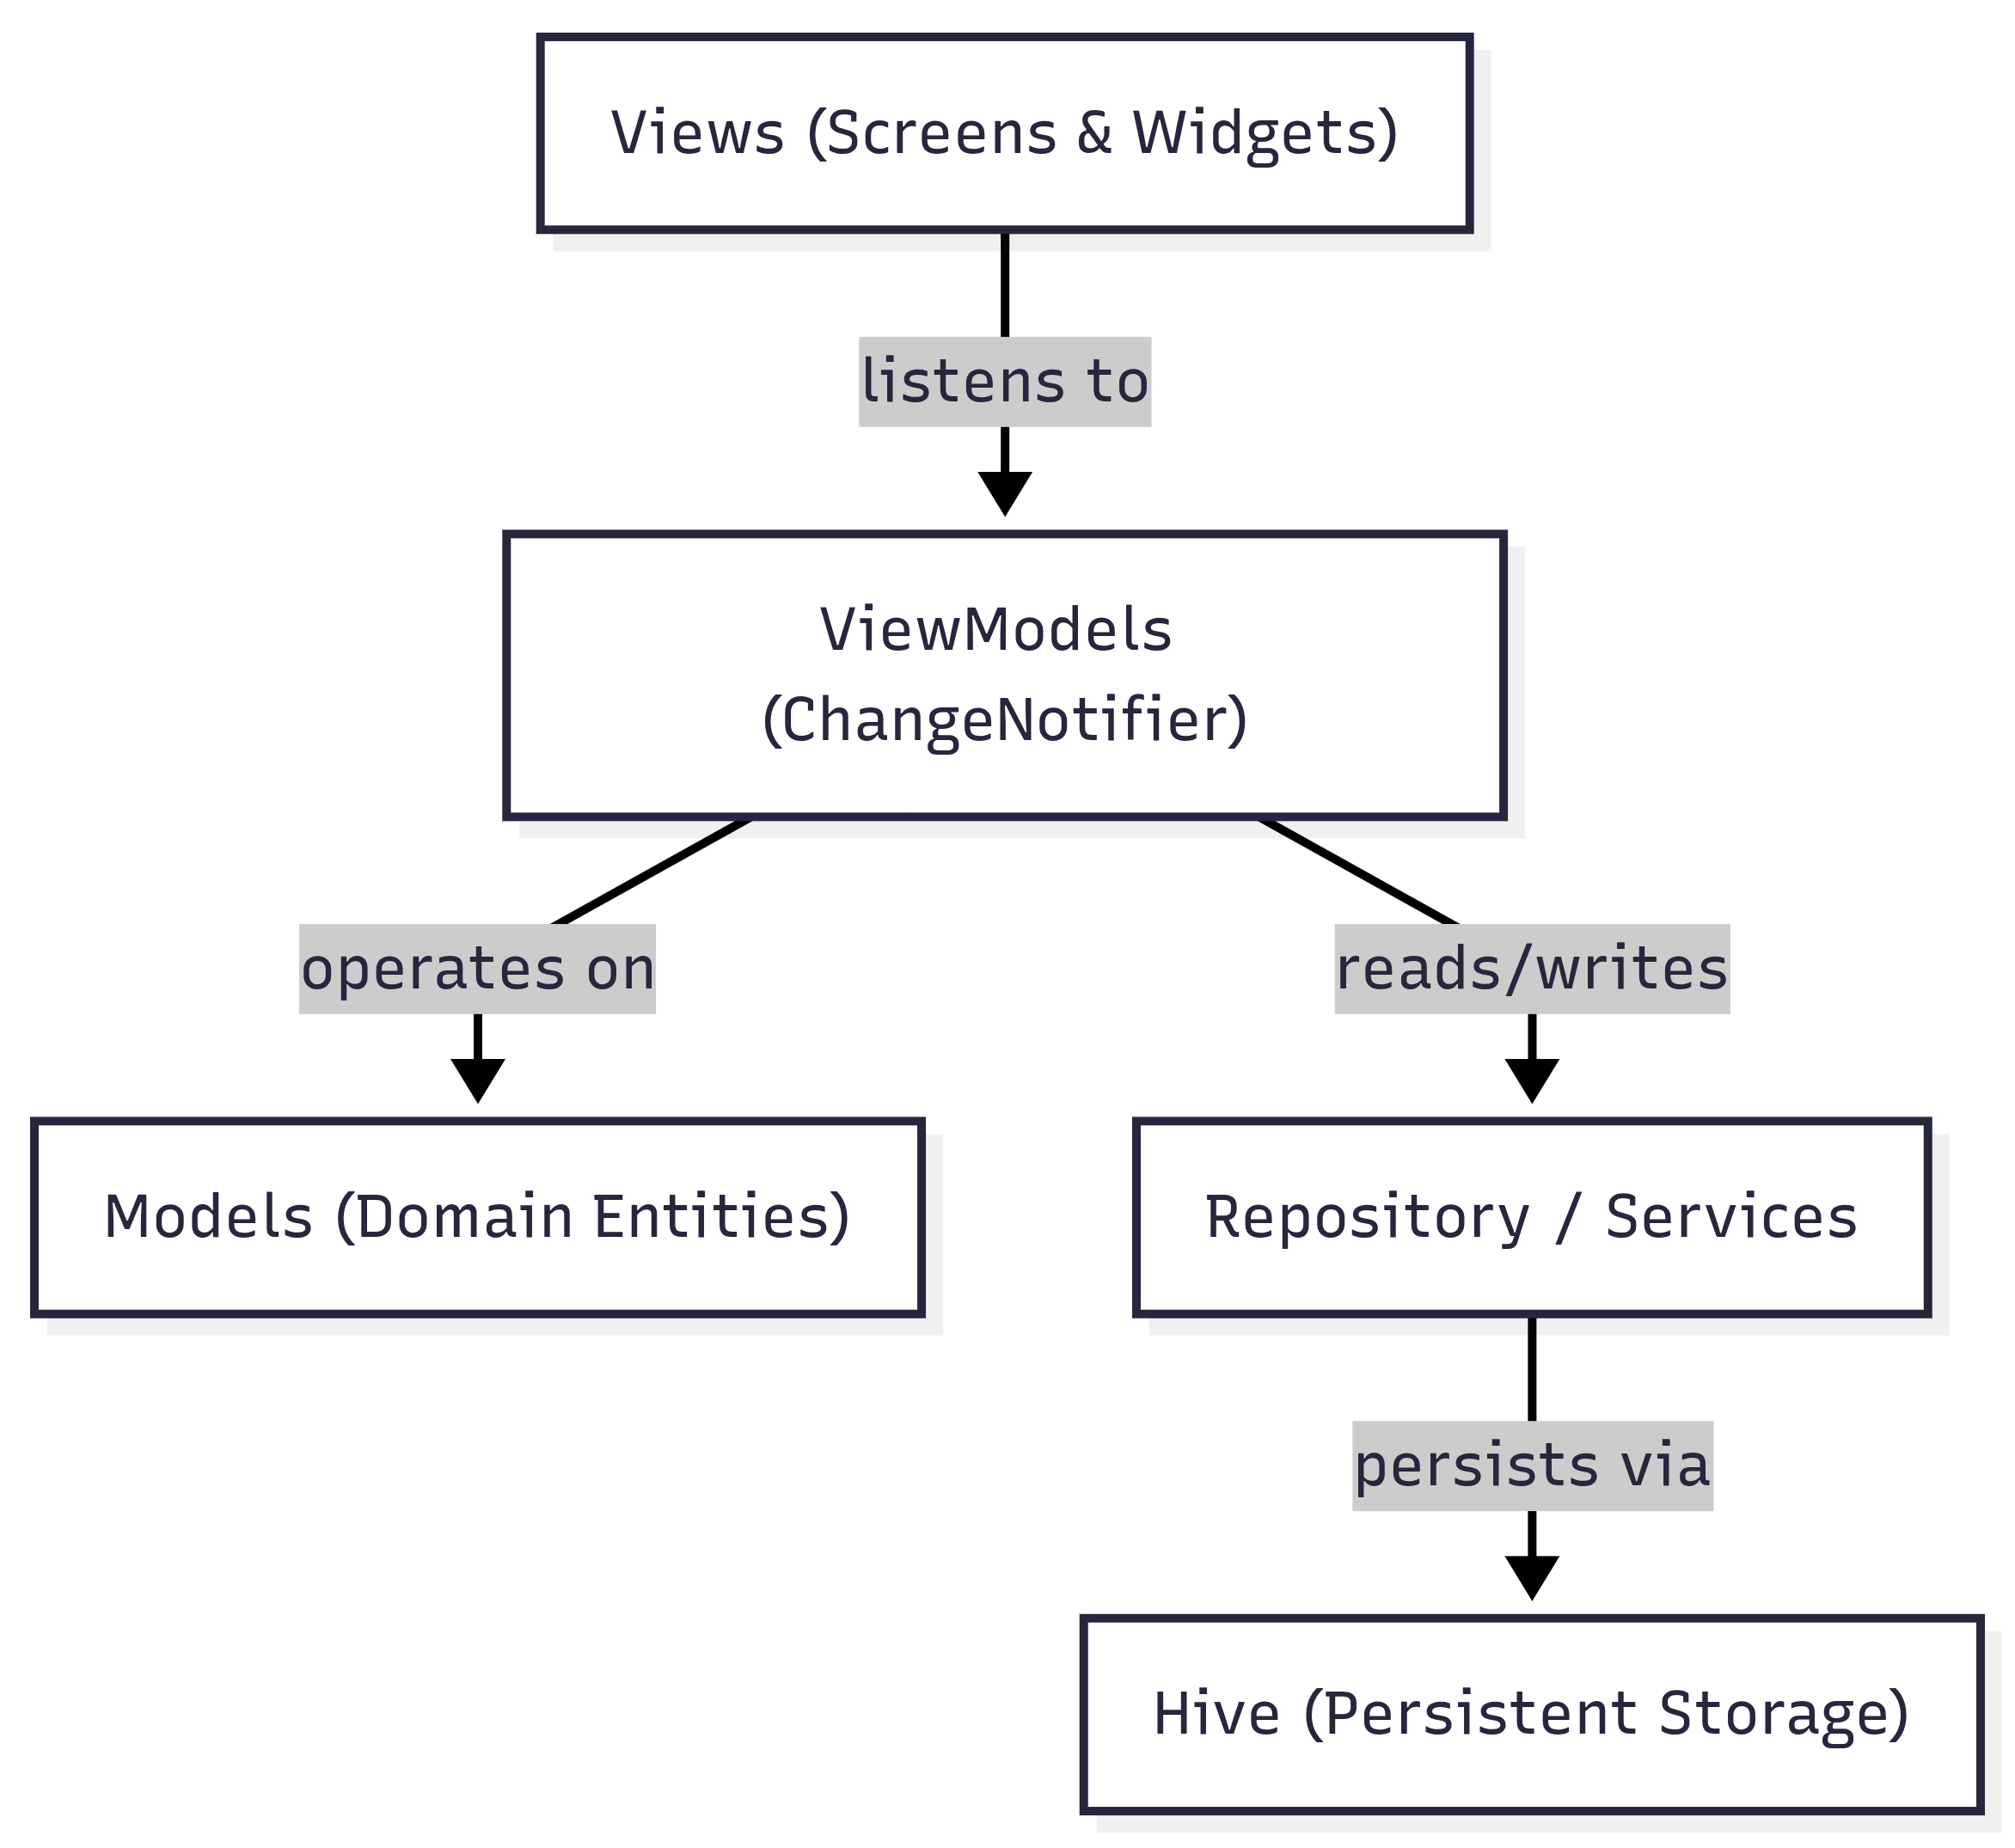
\includegraphics[width=0.7\textwidth]{images/layer-diagram.png}
  \caption{Layer Diagram}
\end{figure}

\subsection{Layer Responsibilities}

\begin{description}[style=nextline]
  \item[Models (\texttt{lib/models/})]
    Pure Dart domain entities with no framework dependencies. Business logic lives in entity methods (e.g.\ \texttt{Order.calculatePointsEarned()}, \texttt{CartItem.calculateSubtotal()}). Constructors use \texttt{assert} for invariant validation.

  \item[ViewModels (\texttt{lib/viewmodels/})]
    State holders extending \texttt{ChangeNotifier}. Each screen has a corresponding ViewModel that manages its state and exposes methods for user actions. ViewModels are manually wired in \texttt{main.dart} and passed as constructor parameters.

  \item[Views (\texttt{lib/views/})]
    \texttt{StatelessWidget} screens that receive their ViewModel via constructor injection. Navigation uses raw \texttt{Navigator.push}.

  \item[Repository (\texttt{lib/repositories/})]
    \texttt{AppRepository} aggregates all ViewModels and coordinates cross-cutting concerns (e.g.\ awarding stamps and points after checkout).

  \item[Services (\texttt{lib/services/})]
    \texttt{LocalStorage} wraps \texttt{Hive} for persisting user profile data, orders, cart items, and loyalty stamp count.
\end{description}

% ══════════════════════════════════════════════════════════
\section{Screens}

The application consists of 8 screens, each mapped to a specification requirement.

\subsection{Home Screen}

Displays a greeting header, the user's loyalty card, and a grid of available coffee products. The bottom navigation bar provides access to all main sections.

\textbf{Interactions:}
\begin{itemize}[nosep]
  \item Tap a product card $\rightarrow$ Navigate to Details Screen
  \item Bottom navigation tabs $\rightarrow$ Navigate to corresponding screen
\end{itemize}

\begin{figure}[H]
  \centering
  \fbox{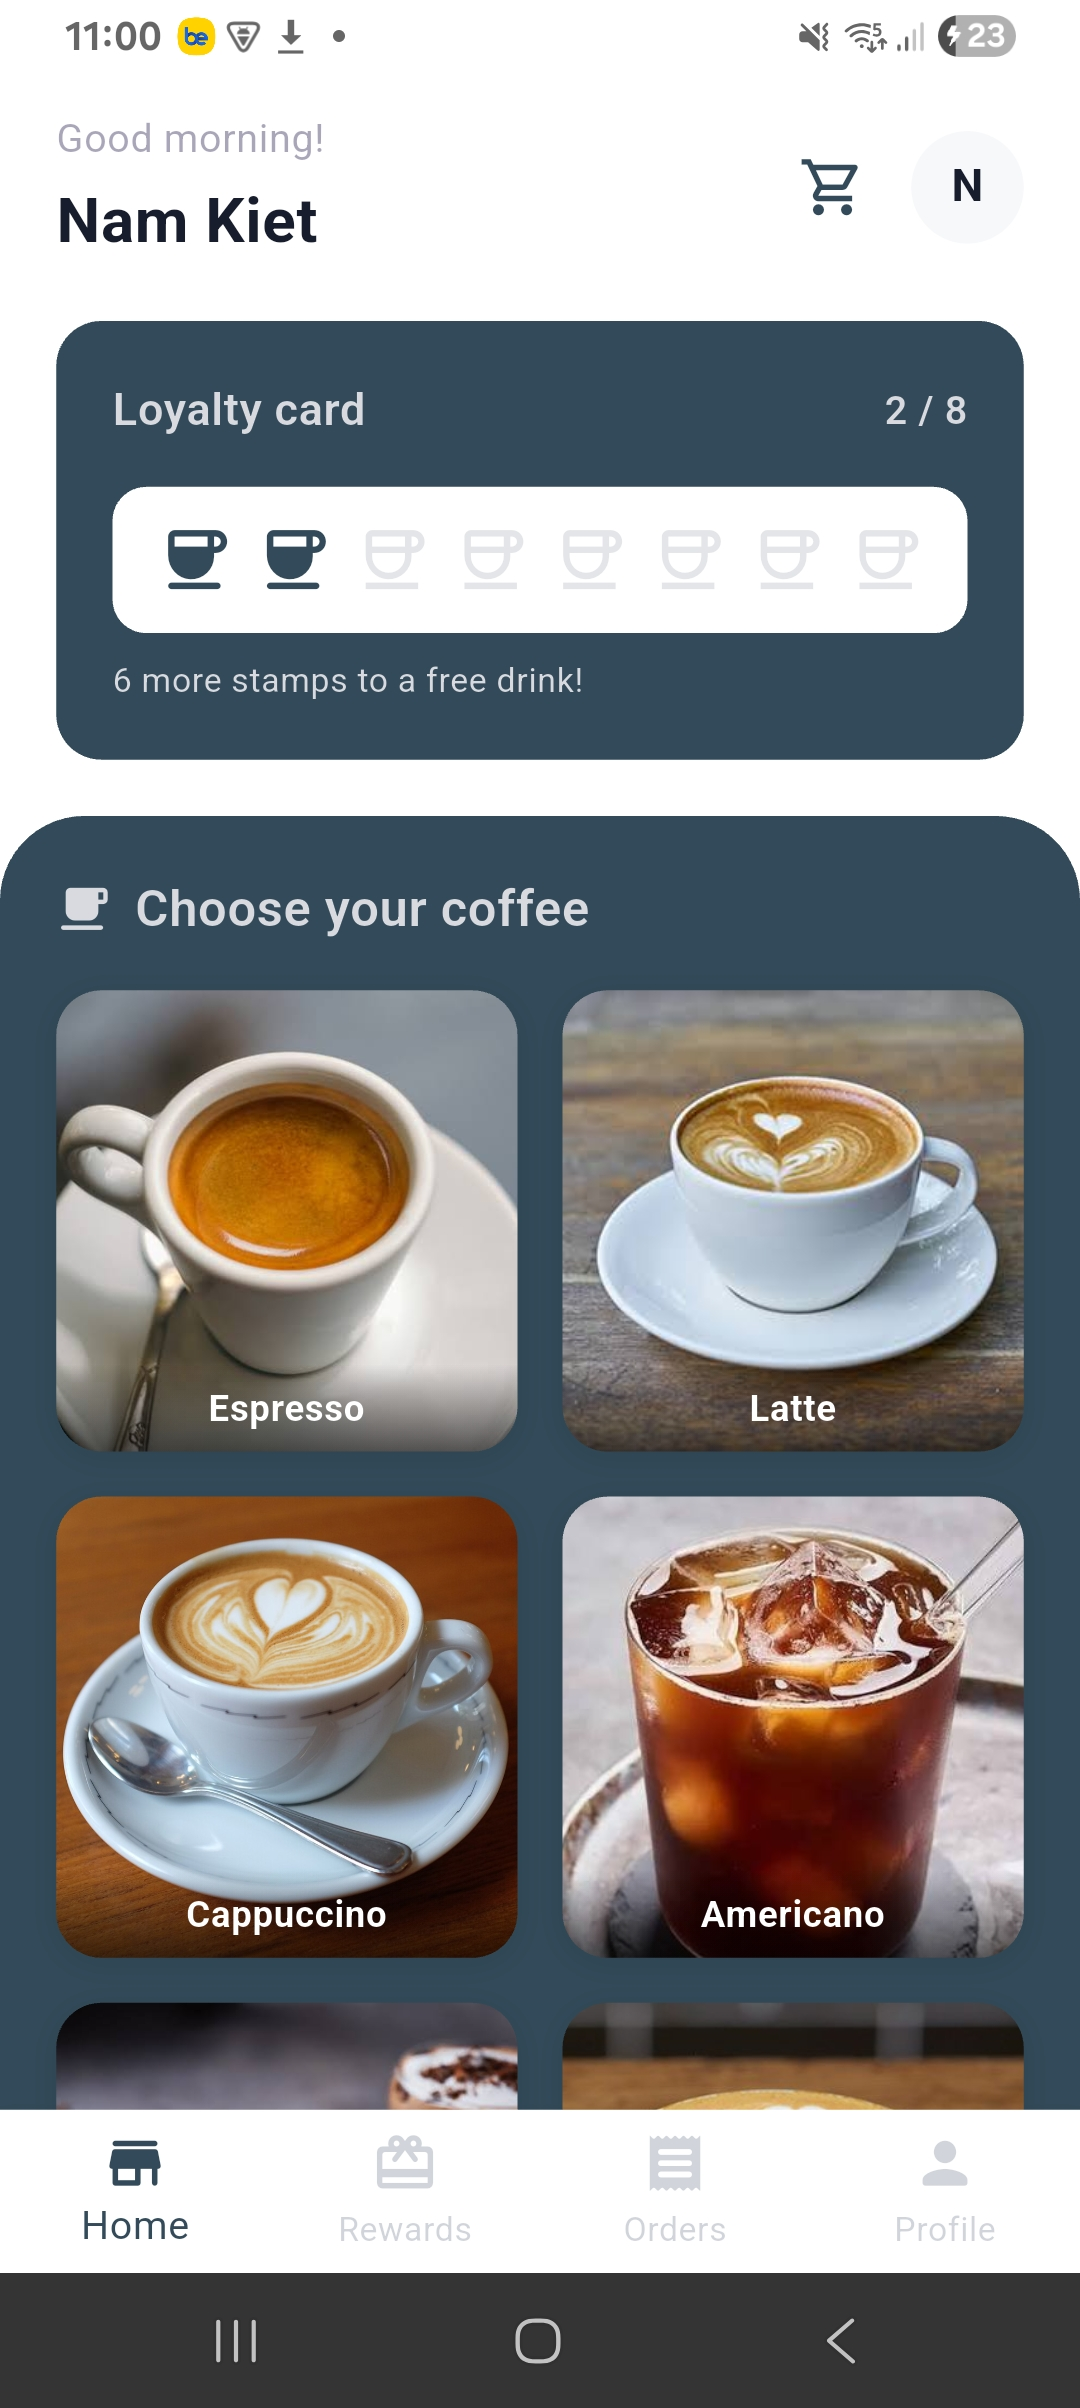
\includegraphics[width=0.4\textwidth]{images/home.jpg}}
  \caption{Home Screen}
\end{figure}

\subsection{Details Screen}

Shows product details with customization options (shot type, size, ice level). Total price updates reactively as options and quantity change.

\textbf{Interactions:}
\begin{itemize}[nosep]
  \item Cart icon $\rightarrow$ Navigate to My Cart
  \item ``Add to Cart'' button $\rightarrow$ Persist item, show centered overlay confirmation
  \item Back button $\rightarrow$ Return to Home
\end{itemize}

\begin{figure}[H]
  \centering
  \fbox{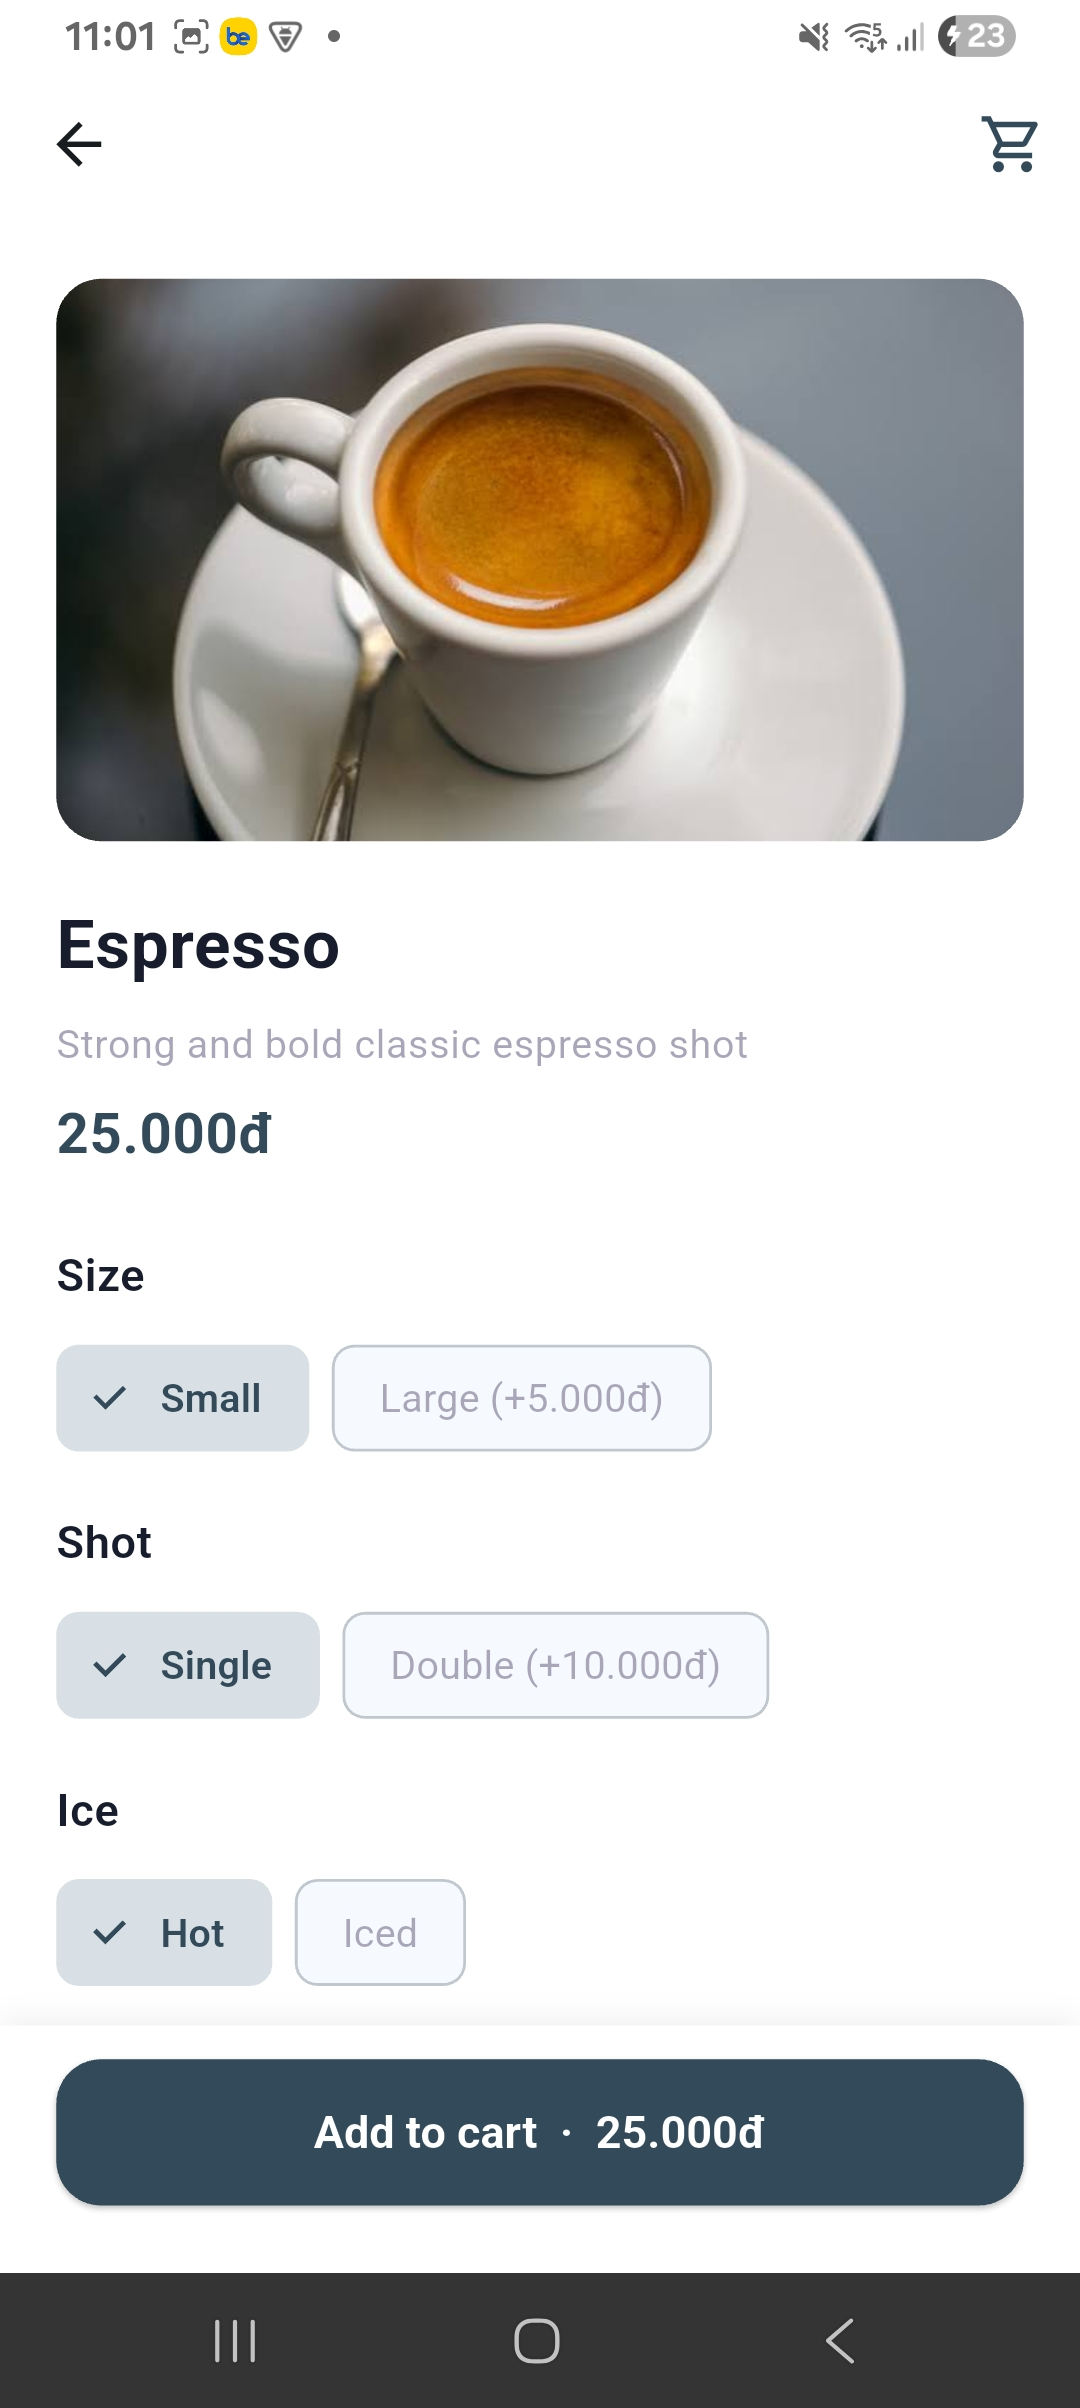
\includegraphics[width=0.4\textwidth]{images/details.jpg}}
  \caption{Details Screen with Customization}
\end{figure}

\subsection{My Cart Screen}

Renders cart items in a list view reflecting selected customizations. Displays the aggregate total price.

\textbf{Interactions:}
\begin{itemize}[nosep]
  \item ``Checkout'' button $\rightarrow$ Navigate to Order Success
  \item Swipe left on item $\rightarrow$ Remove from cart
\end{itemize}

\begin{figure}[H]
  \centering
  \fbox{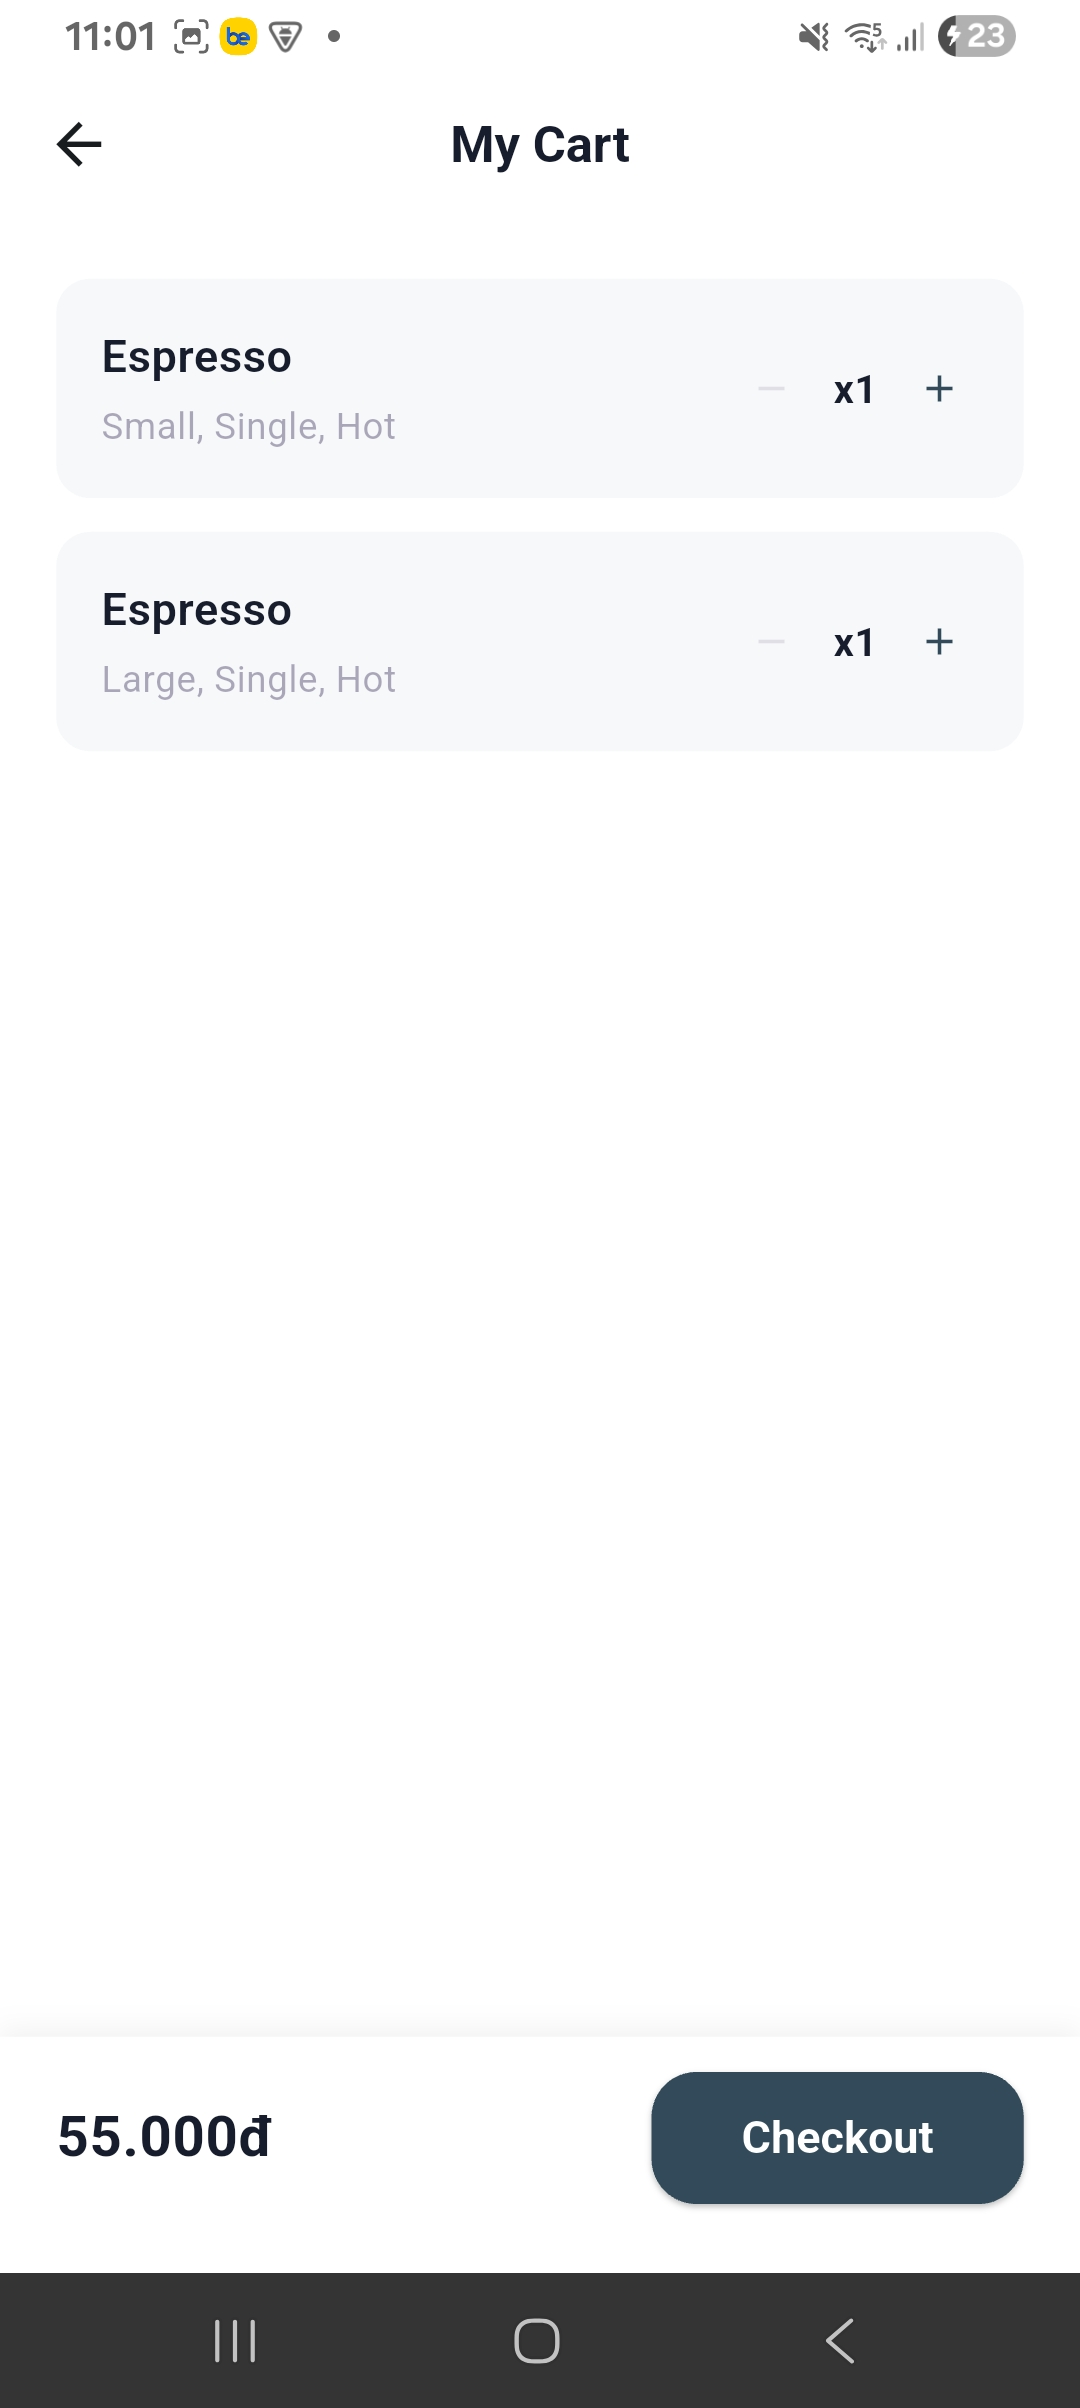
\includegraphics[width=0.4\textwidth]{images/cart.jpg}}
  \caption{My Cart Screen}
\end{figure}

\subsection{Order Success Screen}

Confirms the order was placed successfully.

\textbf{Interactions:}
\begin{itemize}[nosep]
  \item ``Track My Order'' button $\rightarrow$ Navigate to My Orders
\end{itemize}

\begin{figure}[H]
  \centering
  \fbox{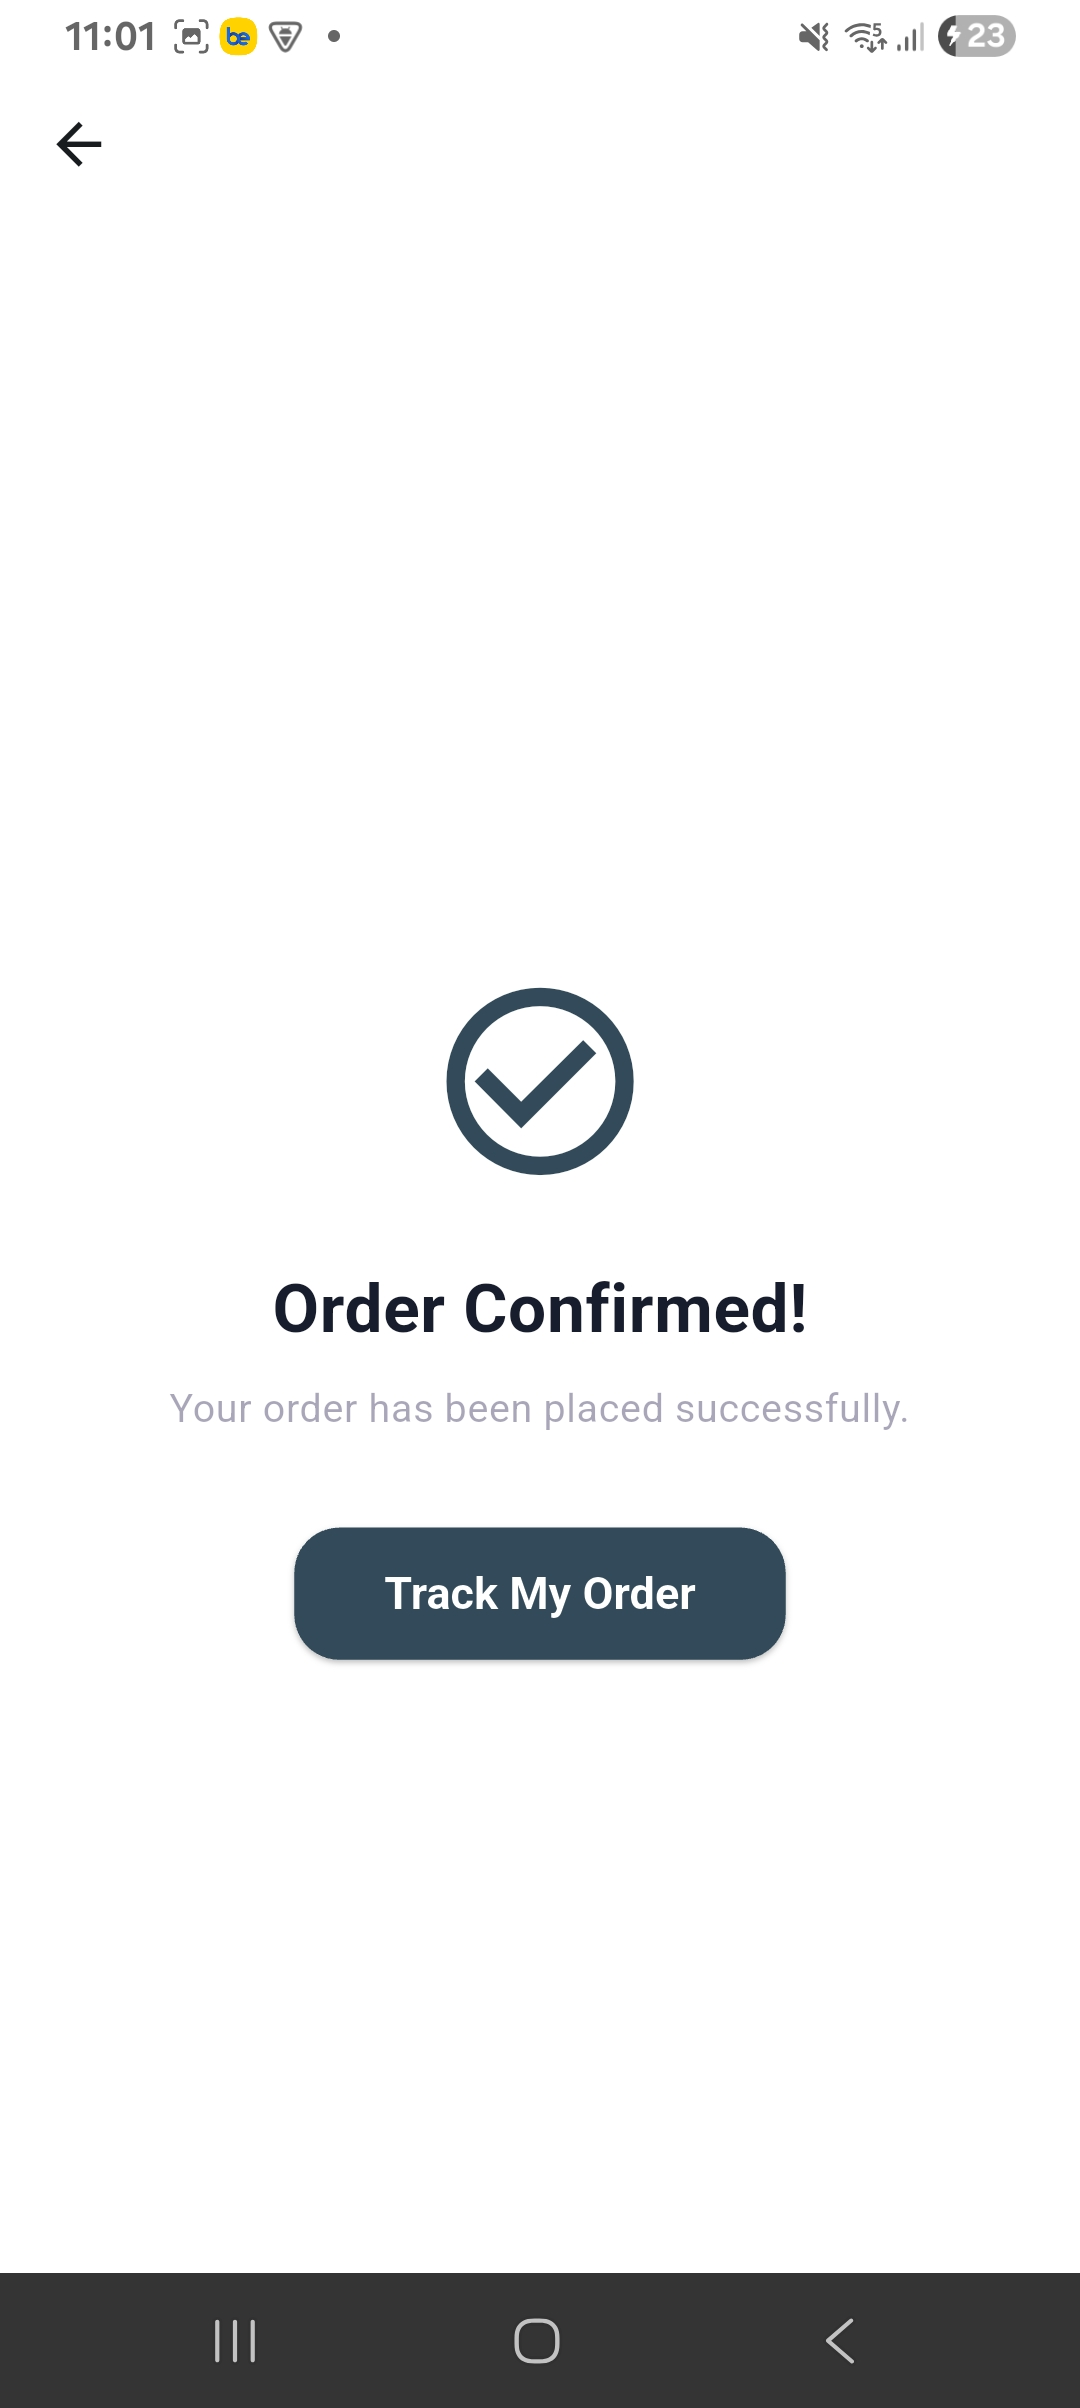
\includegraphics[width=0.4\textwidth]{images/order_success.jpg}}
  \caption{Order Success Screen}
\end{figure}

\subsection{My Orders Screen}

Two-tab layout separating \textbf{Ongoing} and \textbf{History} orders.

\textbf{Interactions:}
\begin{itemize}[nosep]
  \item Tab switching filters the order list
  \item Swipe left on order card $\rightarrow$ Toggle status between ongoing and history
\end{itemize}

\begin{figure}[H]
  \centering
  \fbox{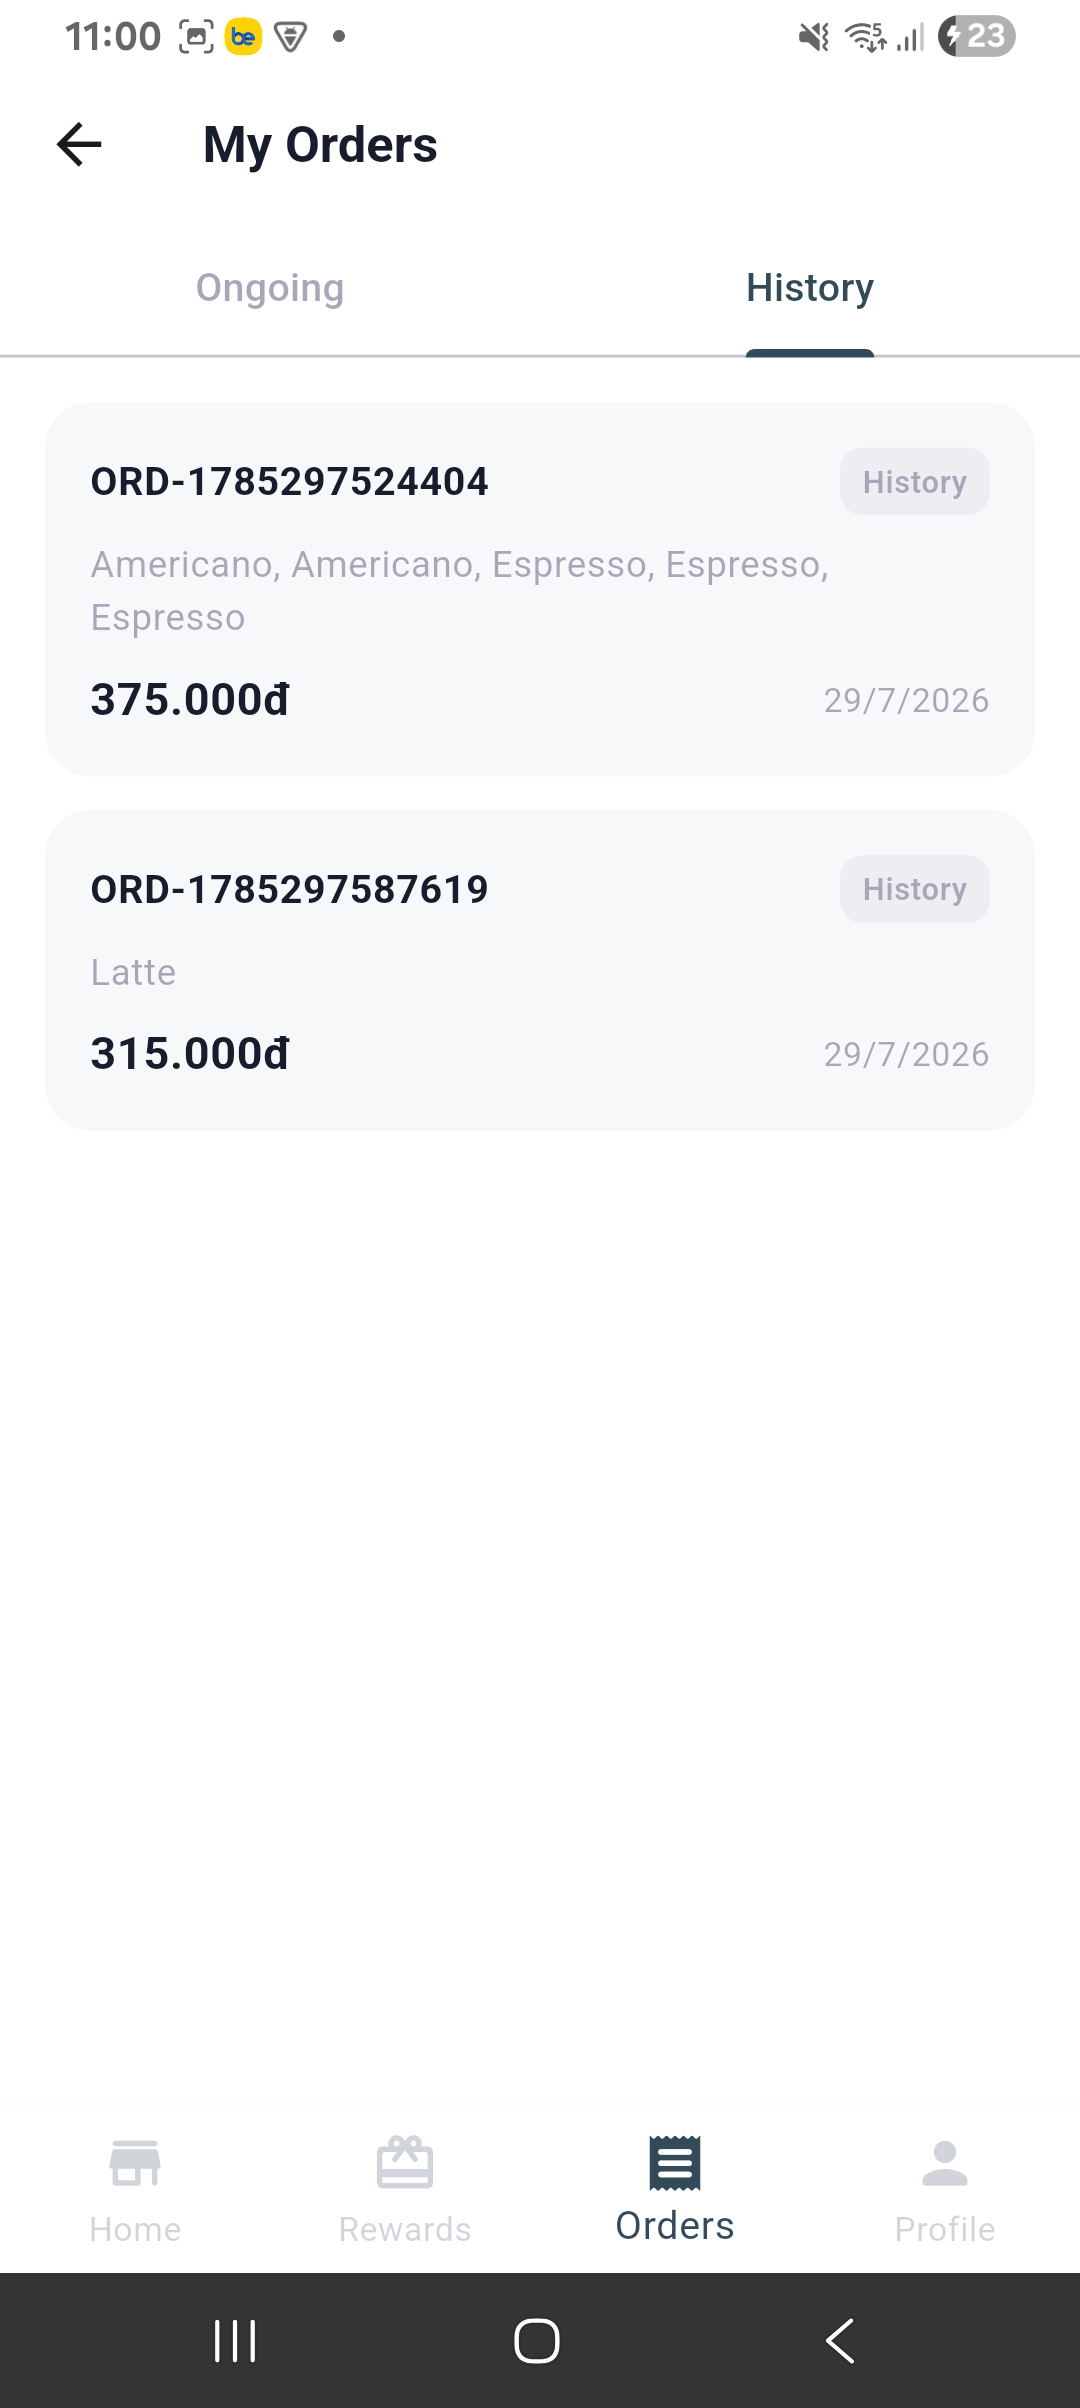
\includegraphics[width=0.4\textwidth]{images/orders.jpg}}
  \caption{My Orders Screen}
\end{figure}

\subsection{Rewards Screen}

Displays the loyalty card with current stamp count, total reward points, and transaction history.

\textbf{Interactions:}
\begin{itemize}[nosep]
  \item Tap loyalty card at 8 stamps $\rightarrow$ Reset to 0
  \item Redeem button $\rightarrow$ Navigate to Redeem Rewards Screen
\end{itemize}

\textbf{Business rules:}
\begin{itemize}[nosep]
  \item $+1$ stamp per completed order, maximum 8
  \item Points awarded: $\lfloor \text{orderTotal} / 10{,}000 \rfloor$
\end{itemize}

\begin{figure}[H]
  \centering
  \fbox{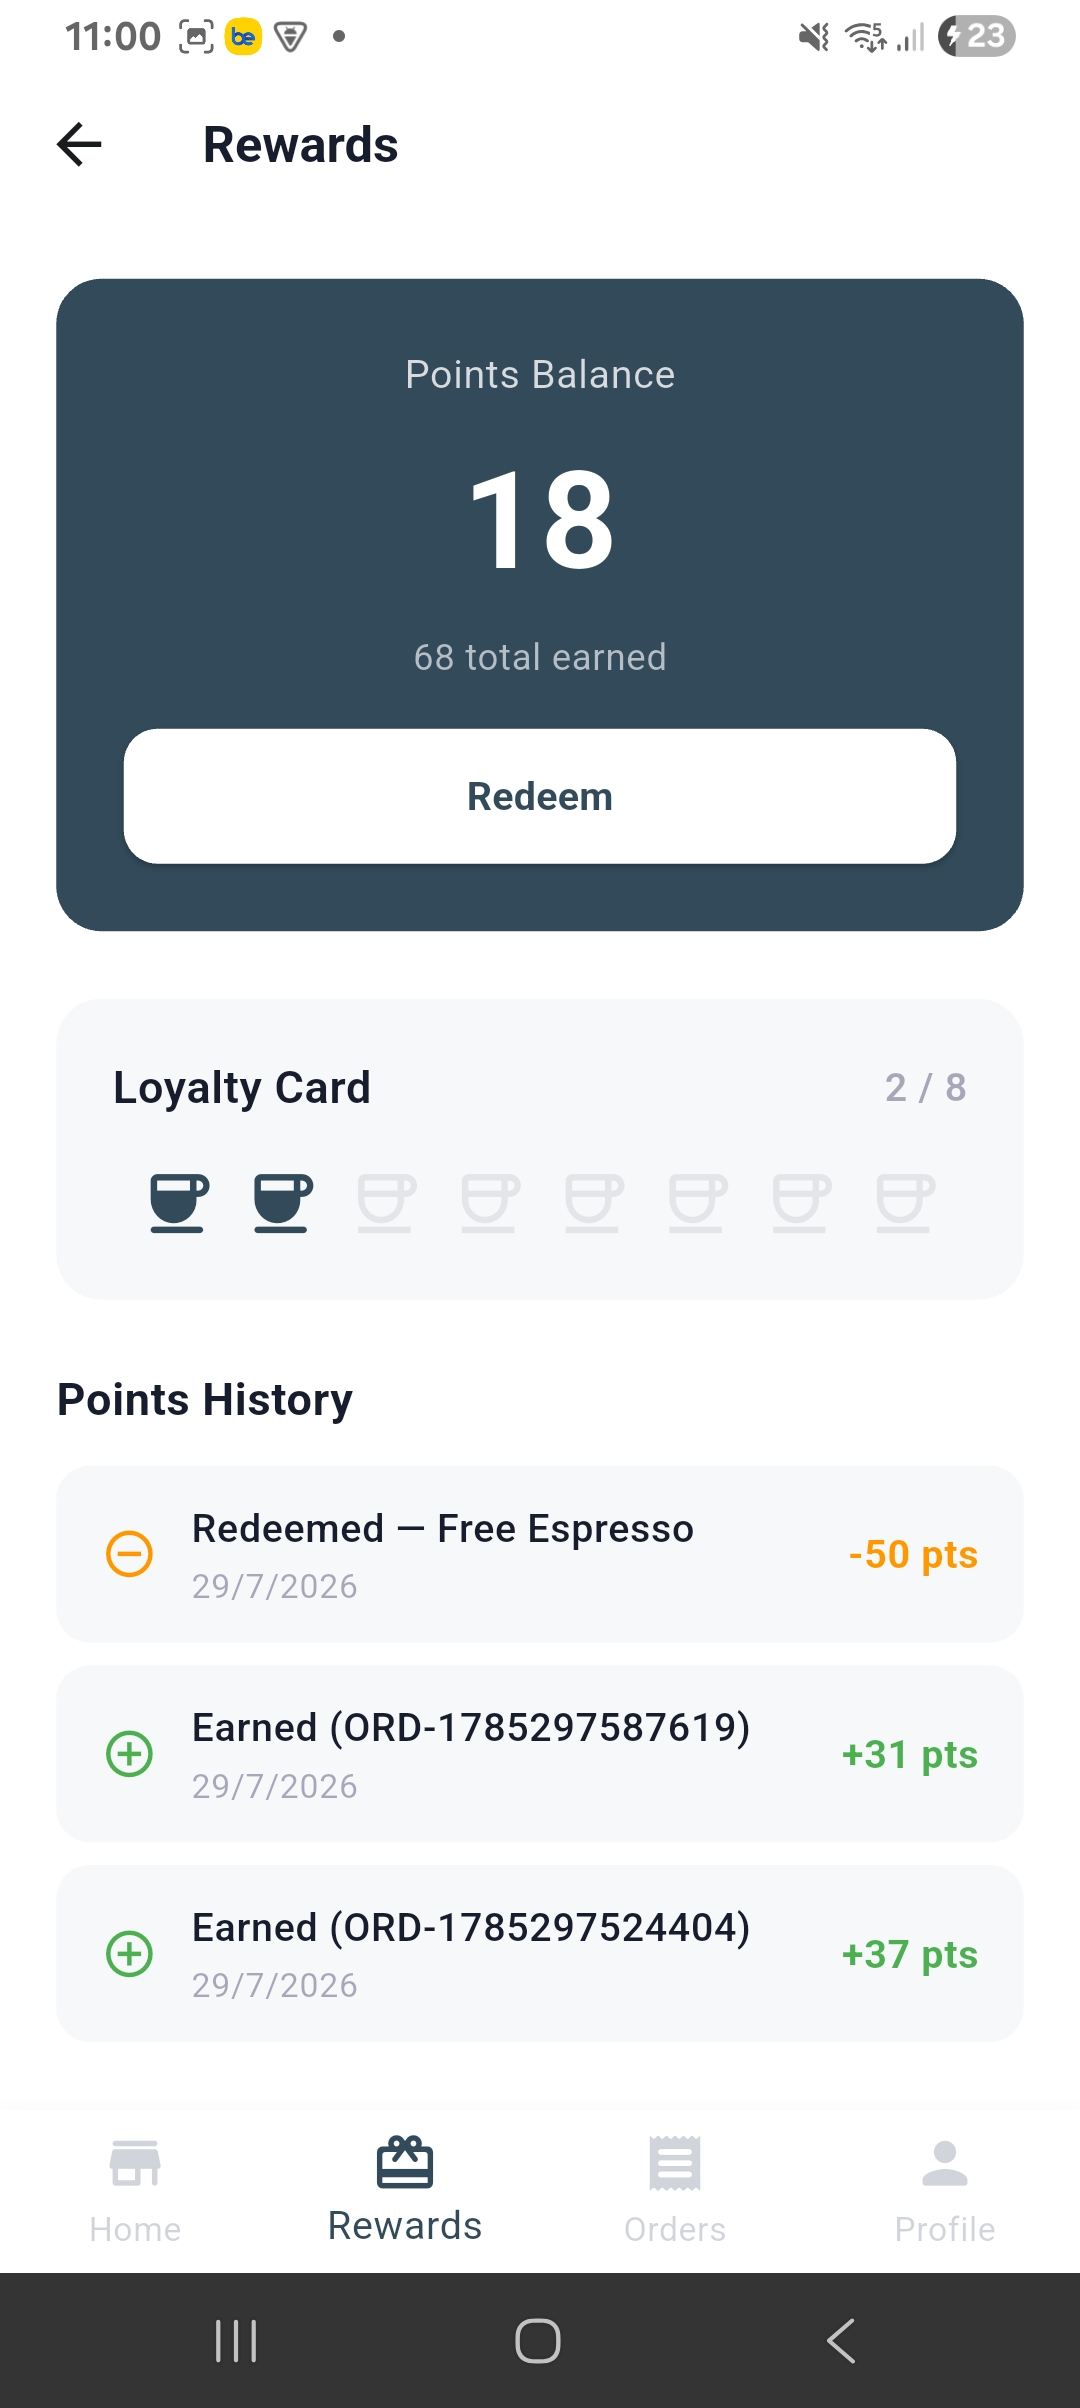
\includegraphics[width=0.4\textwidth]{images/rewards.jpg}}
  \caption{Rewards Screen}
\end{figure}

\subsection{Redeem Rewards Screen}

Product catalog showing items available for point redemption. Tapping an item shows a confirmation dialog; confirming deducts points from the balance.

\begin{figure}[H]
  \centering
  \fbox{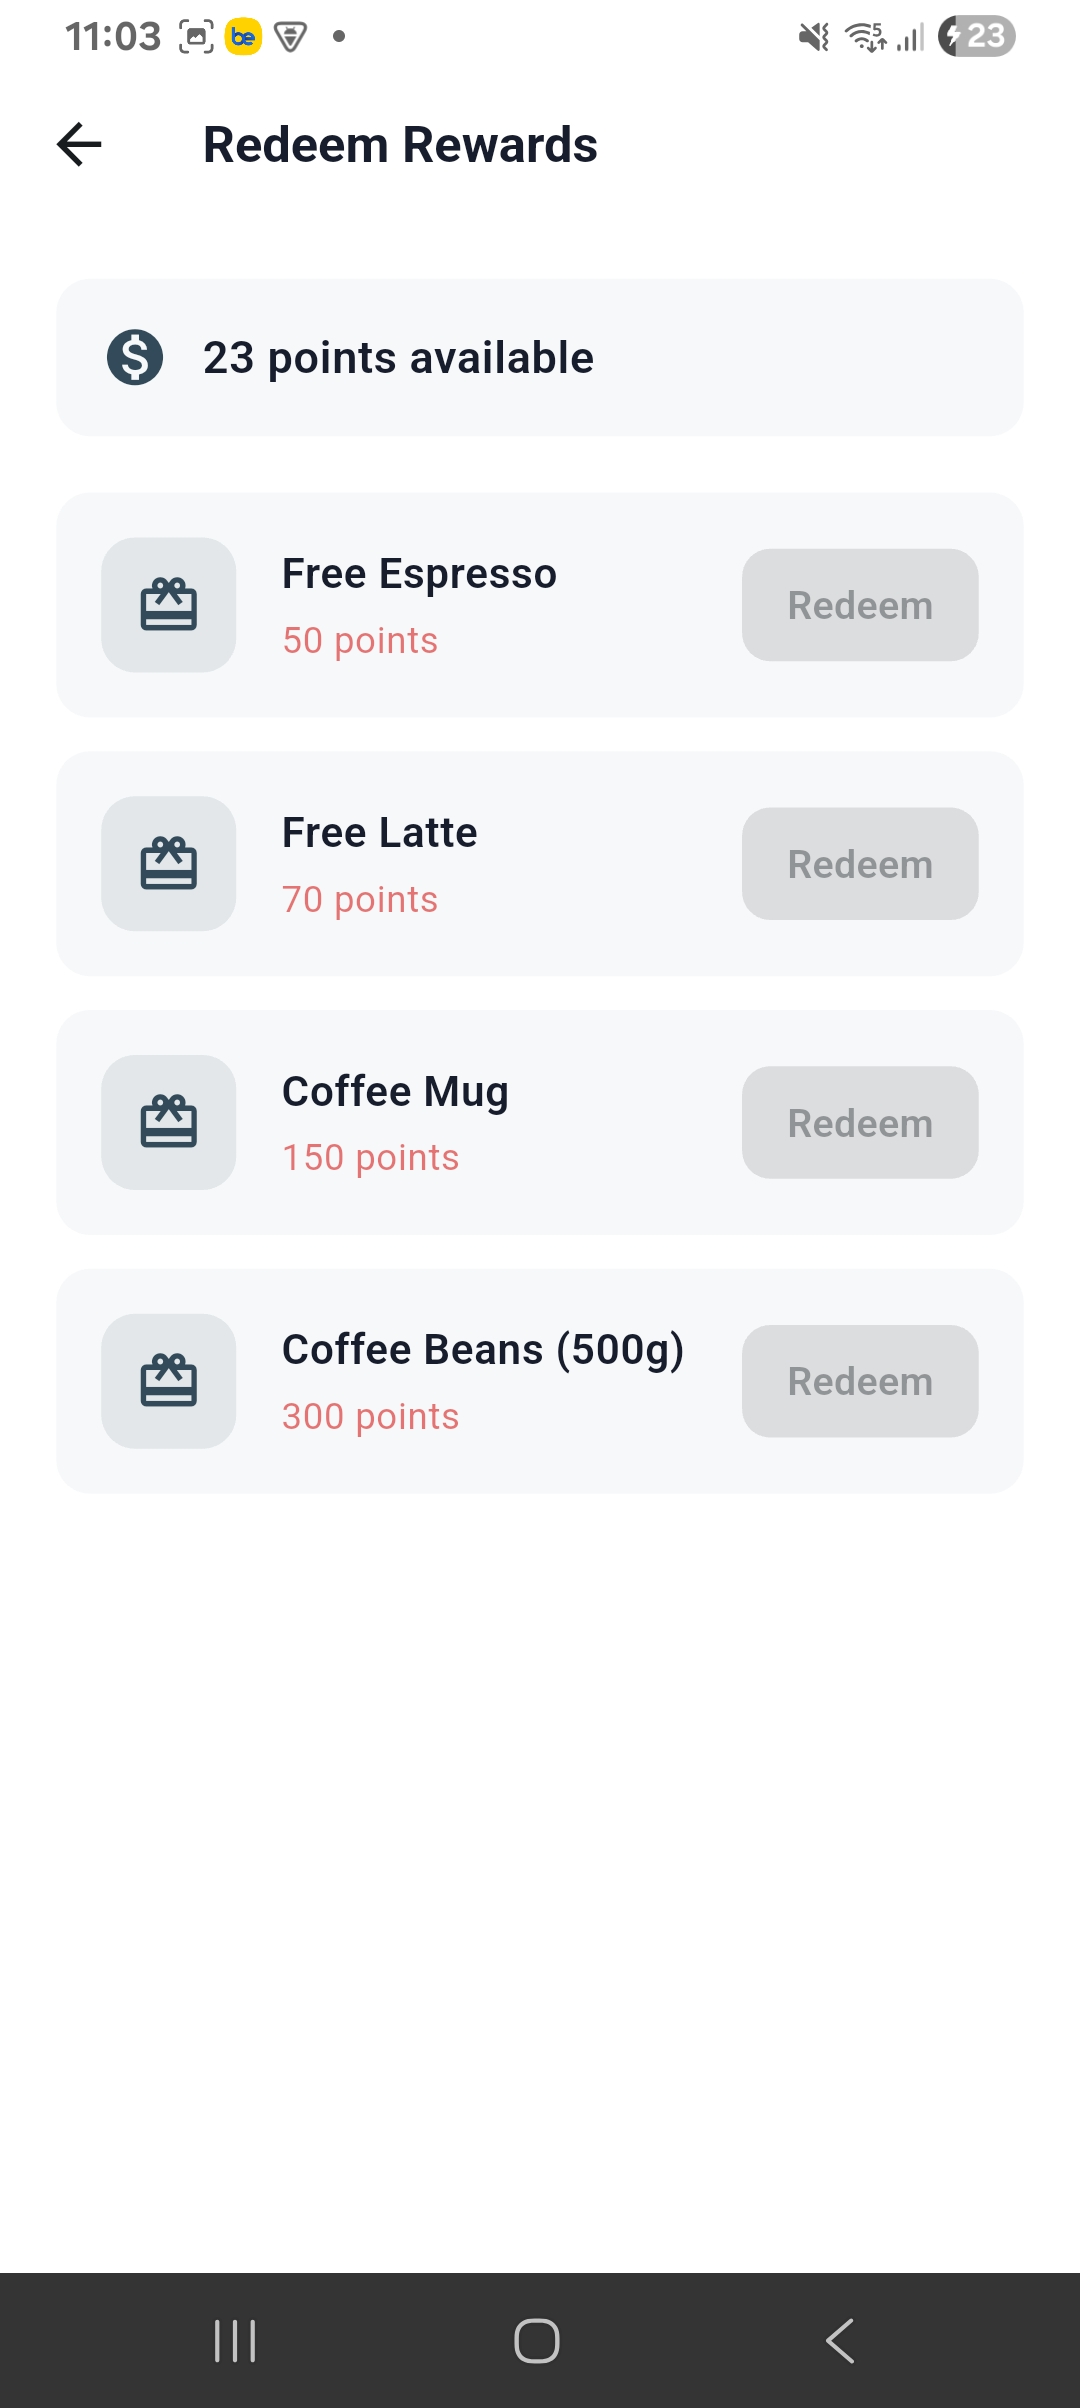
\includegraphics[width=0.4\textwidth]{images/redeem.jpg}}
  \caption{Redeem Rewards Screen}
\end{figure}

\subsection{Profile Screen}

Displays user profile (name, email, phone, address, avatar). An edit icon toggles inline editing; changes are persisted via \texttt{Hive}.

\begin{figure}[H]
  \centering
  \fbox{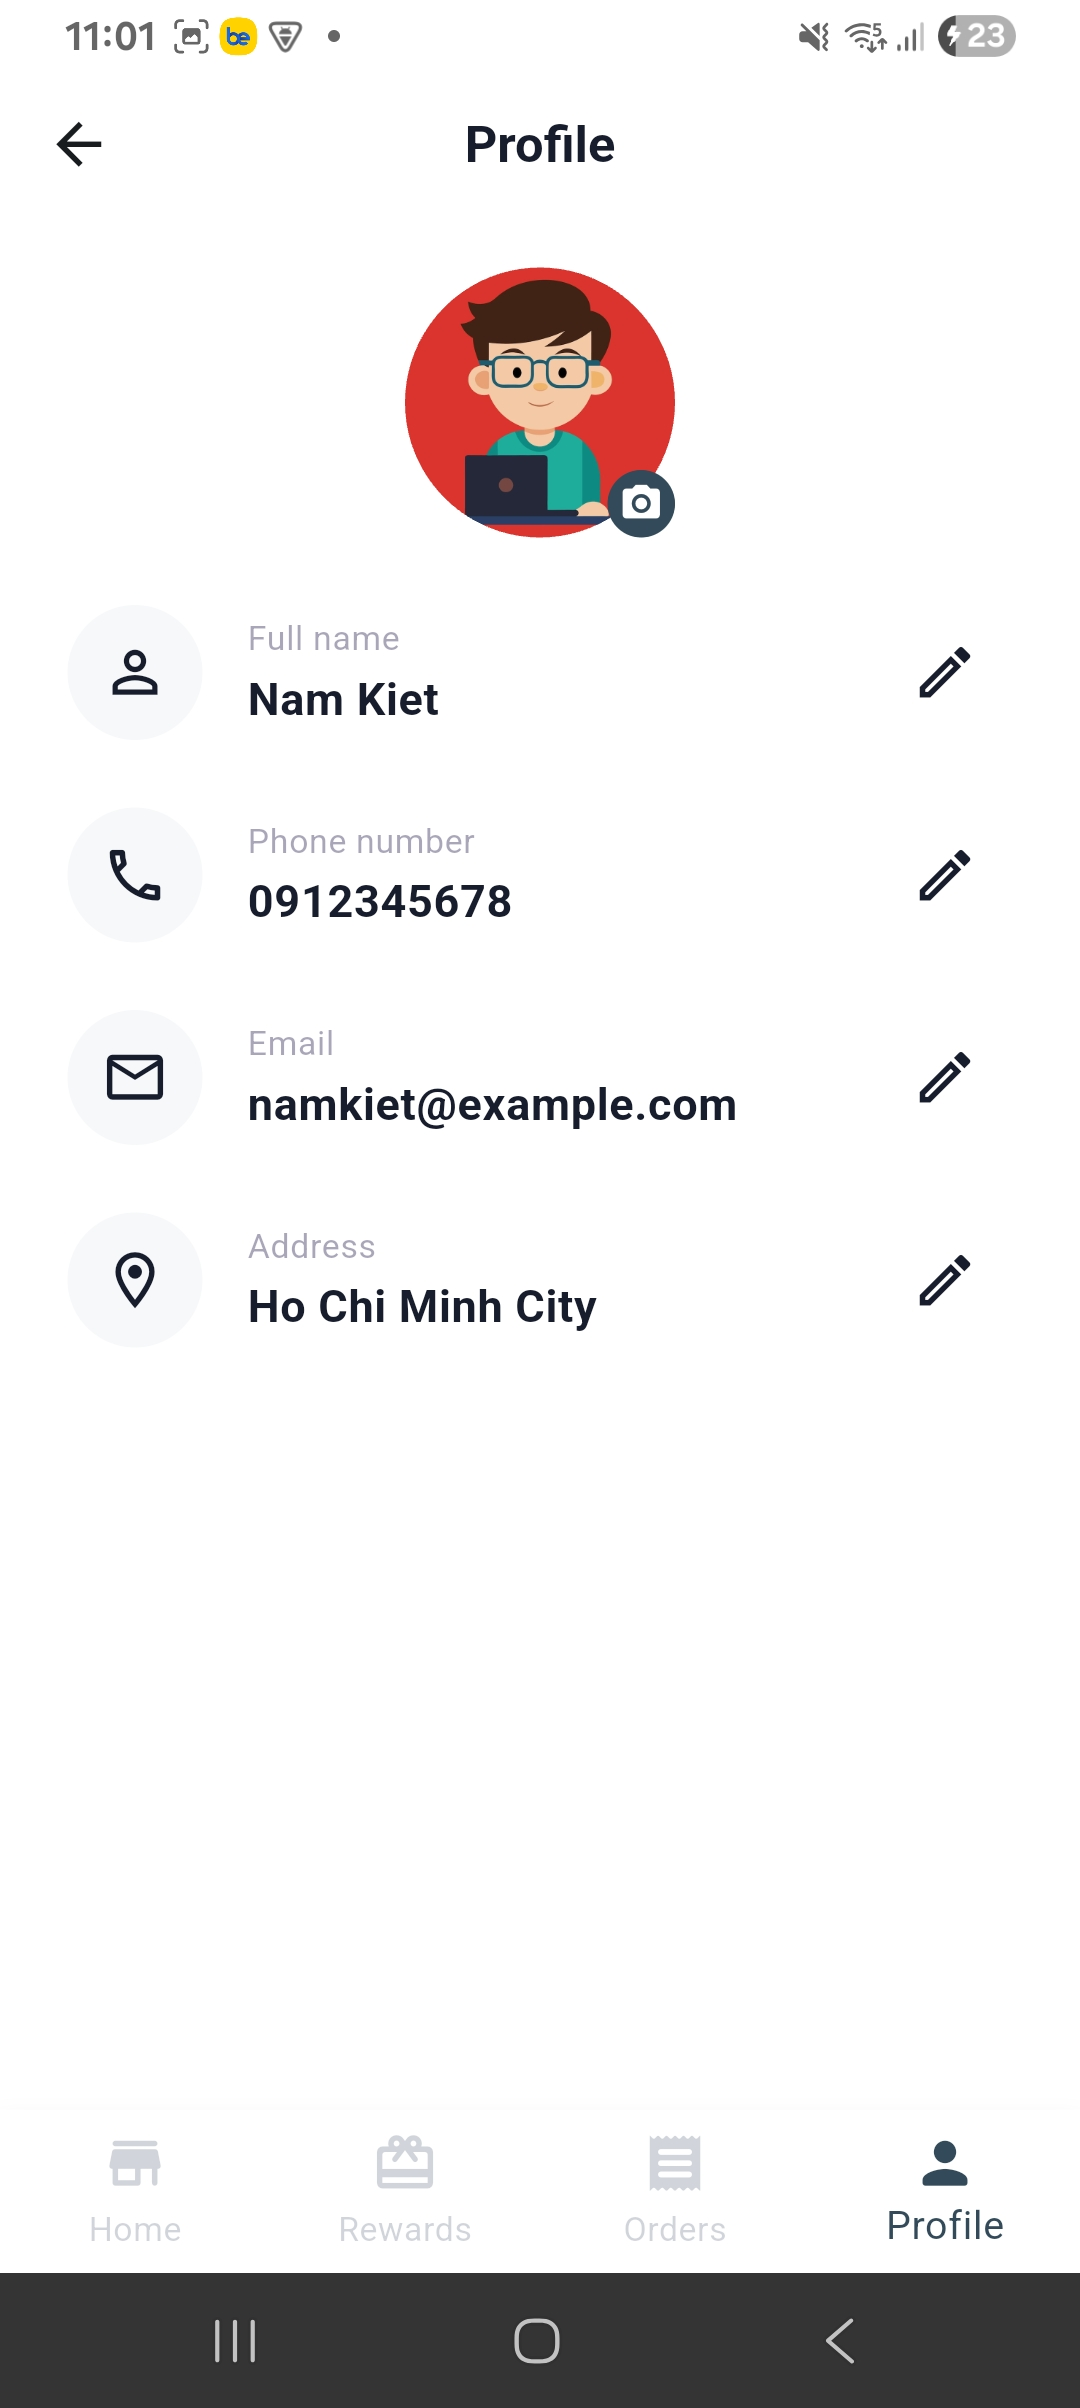
\includegraphics[width=0.4\textwidth]{images/profile.jpg}}
  \caption{Profile Screen}
\end{figure}

% ══════════════════════════════════════════════════════════
\section{Domain Model}

\subsection{Entity Overview}

\begin{figure}[H]
  \centering
  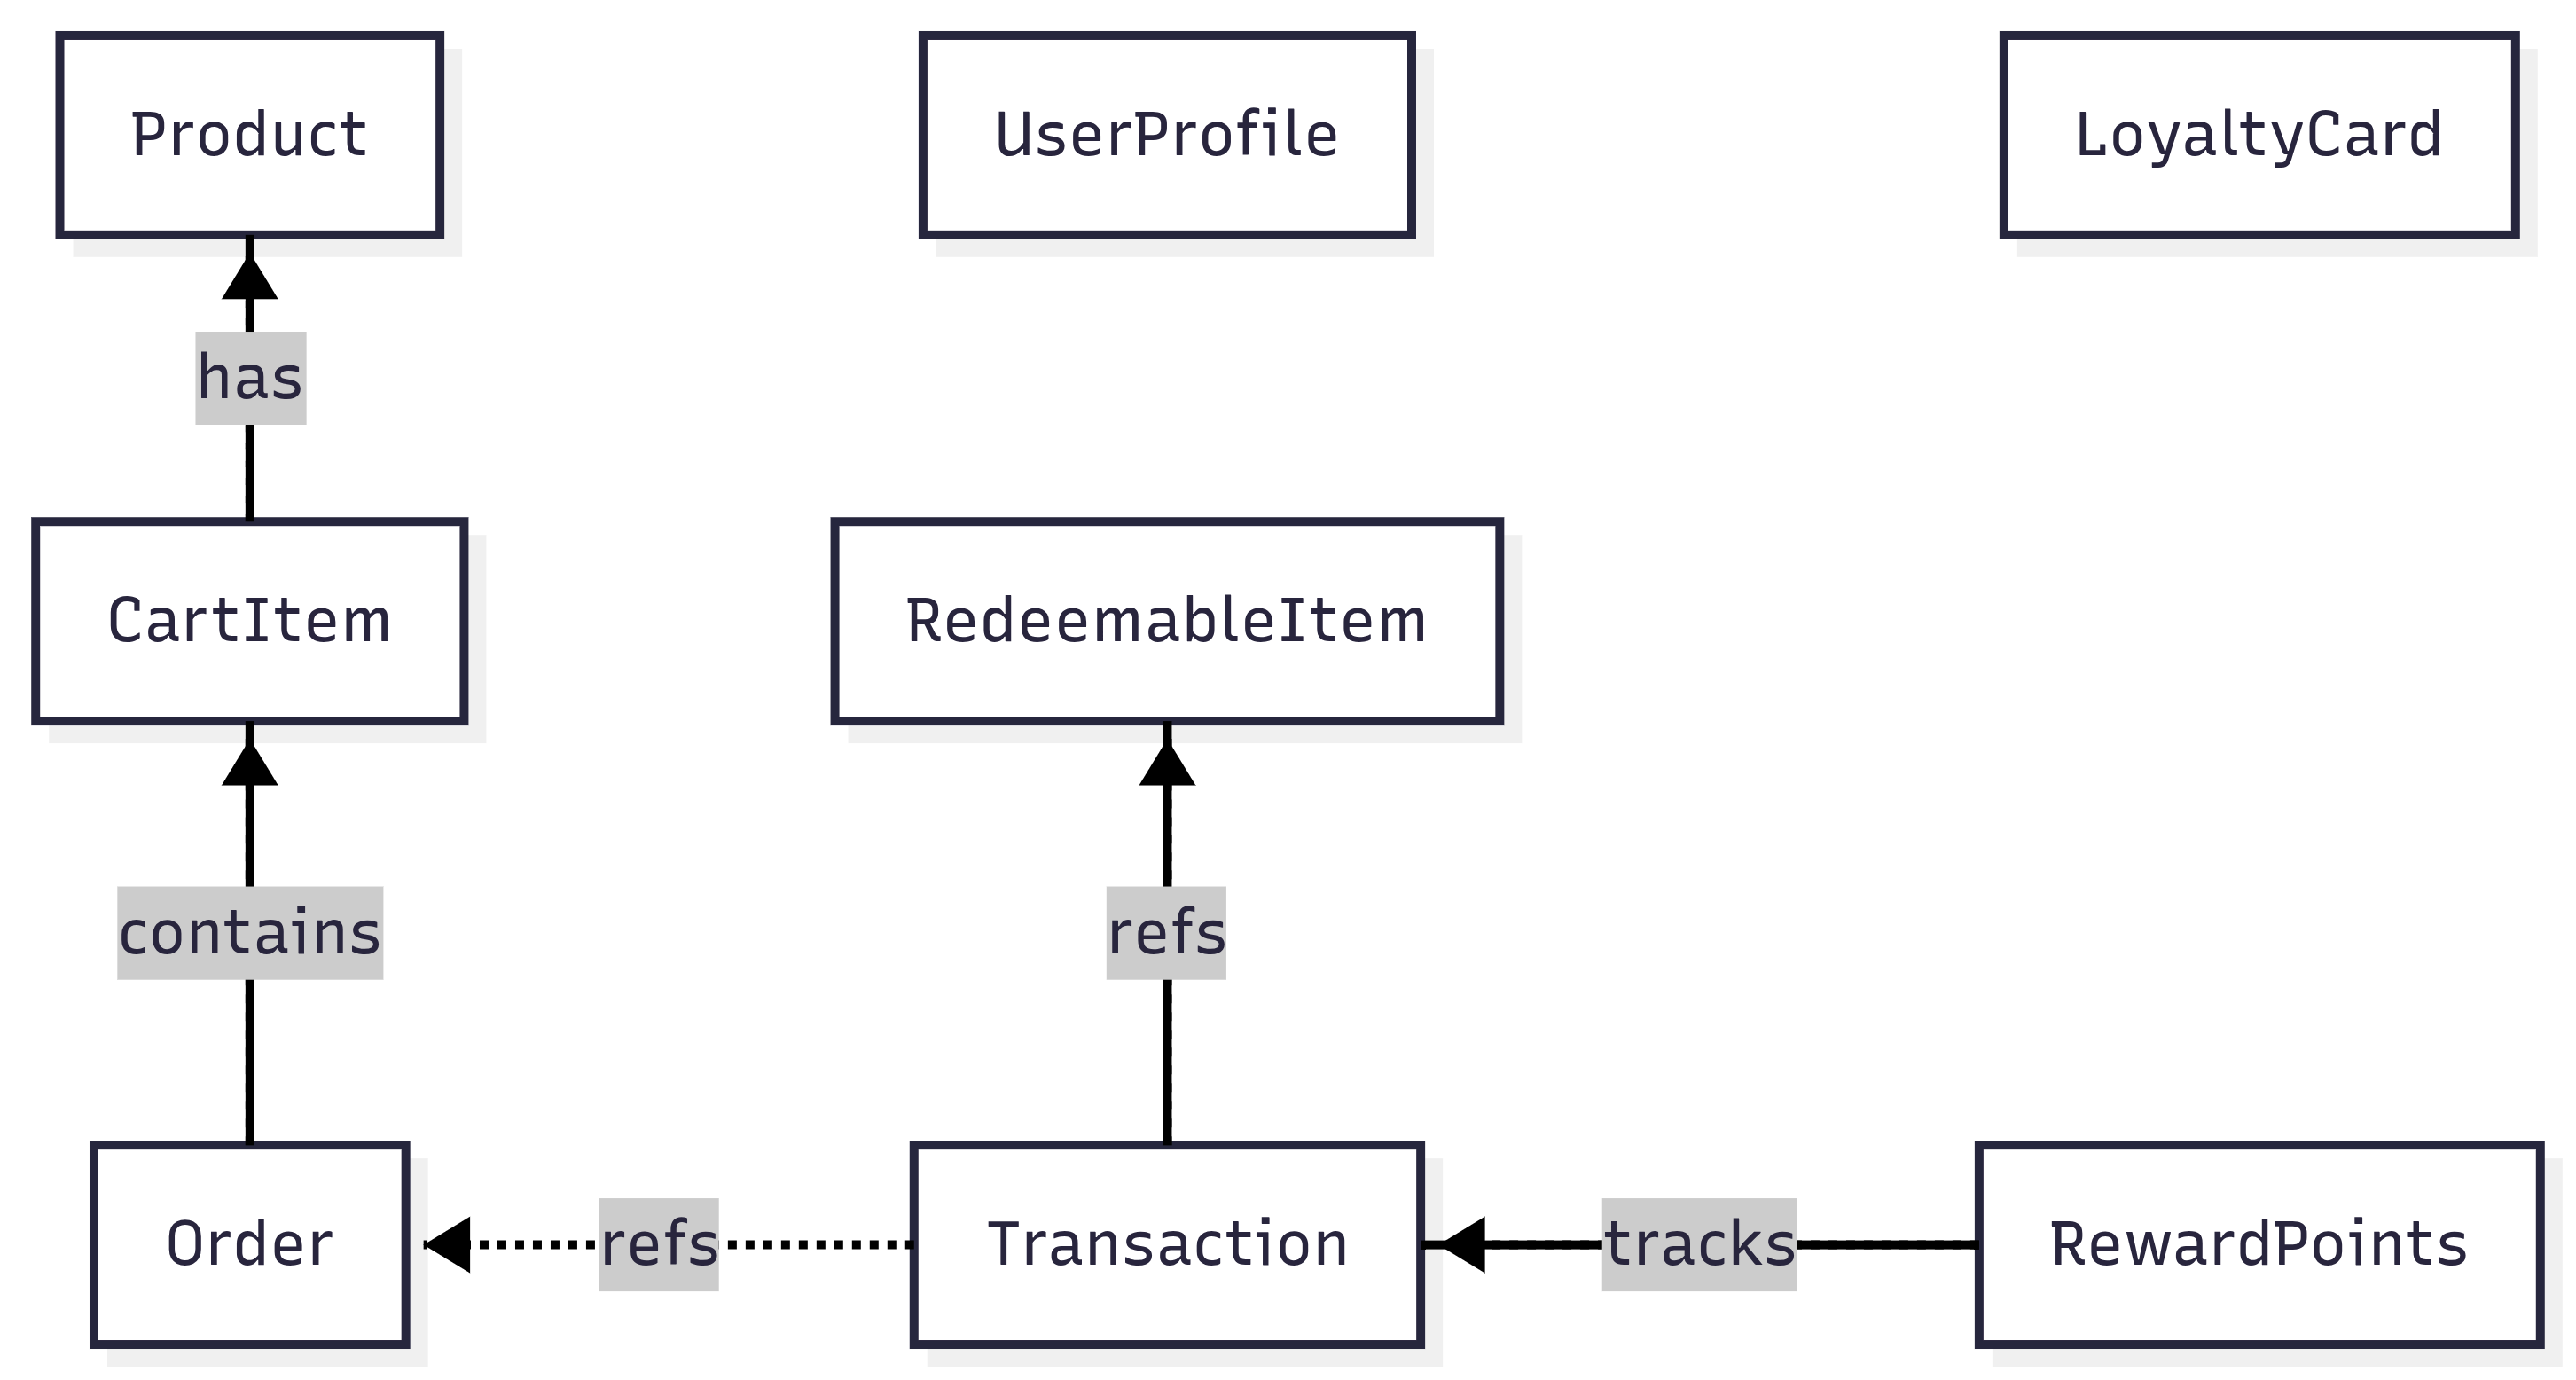
\includegraphics[width=0.8\textwidth]{images/entity-overview.png}
  \caption{Entity Overview}
\end{figure}

\subsection{Entity Details}

\begin{table}[H]
\centering
\begin{tabular}{|p{3cm}|>{\raggedright\arraybackslash}p{4.6cm}|p{7.9cm}|}
  \hline
  \textbf{Entity} & \textbf{Key Attributes} & \textbf{Business Logic} \\
  \hline

  Product &
    id, name, basePrice, availableCustomizations &
    Unit price = basePrice + sum of selected customization deltas \\
  \hline

  CartItem &
    product, selectedCustomizations, quantity &
    \texttt{calculateSubtotal()} = unit price $\times$ quantity \\
  \hline

  Order &
    id, items, status, createdAt &
    \texttt{calculateTotalPrice()} = $\sum$ item subtotals \newline
    \texttt{calculatePointsEarned()} = total $\div$ 10{,}000 \\
  \hline

  LoyaltyCard &
    stampCount (0--8) &
    Increment capped at 8; reset only when exactly 8 \\
  \hline

  RewardPoints &
    balance, transactions &
    \texttt{calculateTotalEarned()} = sum of earn transactions \newline
    Redemption rejected if insufficient balance \\
  \hline

  Transaction &
    type (earn/redeem), amount, createdAt &
    References orderId or redeemableItemId \\
  \hline

  RedeemableItem &
    id, name, pointCost &
    Catalog item for point redemption \\
  \hline

  UserProfile &
    name, email, phone, avatarUrl &
    \begin{tabular}[t]{@{}p{\linewidth}@{}}
      • Name must be non-empty\\
      • Email validated by regex\\
      • Phone (optional) must match VN format \texttt{0[35789]\textbackslash d\{8\}}
    \end{tabular} \\
  \hline
\end{tabular}
\caption{Entity Details}
\end{table}

\section{Project Structure}

\begin{lstlisting}[language={},caption={Directory layout}]
lib/
  main.dart
  constants/app_colors.dart
  data/seed_data.dart
  models/
    product.dart        cart_item.dart
    order.dart          loyalty_card.dart
    reward_points.dart  transaction.dart
    redeemable_item.dart  user_profile.dart
  services/local_storage.dart
  repositories/app_repository.dart
  navigation/app_navigator.dart
  utils/format.dart
  viewmodels/
    home_viewmodel.dart     cart_viewmodel.dart
    orders_viewmodel.dart   rewards_viewmodel.dart
    profile_viewmodel.dart  app_view_models.dart
    repo_view_model.dart    ui_models.dart
  views/
    home_screen.dart        details_screen.dart
    cart_screen.dart         orders_screen.dart
    order_success_screen.dart  rewards_screen.dart
    redeem_rewards_screen.dart  profile_screen.dart
  widgets/
    app_chrome.dart         app_scope.dart
    common_blocks.dart      list_tiles.dart
    product_blocks.dart     loyalty_card_block.dart
    blocks/loyalty_card_block.dart
    blocks/product_grid_card.dart

tests/
  unit/
    product_test.dart       cart_item_test.dart
    order_test.dart         loyalty_card_test.dart
    reward_points_test.dart transaction_test.dart
    redeemable_item_test.dart  user_profile_test.dart
    logic_test.dart         integration_test.dart
  ui/
    test_app.dart           home_screen_test.dart
    details_screen_test.dart  cart_screen_test.dart
    orders_screen_test.dart rewards_screen_test.dart
    profile_screen_test.dart
    profile_screen_edit_test.dart
\end{lstlisting}

\section{Testing}

All tests use the built-in \texttt{flutter\_test} framework with no external testing dependencies.

\subsection{Test Summary}

\begin{table}[H]
\centering
\caption{Test results}
\begin{tabular}{lrrr}
  \toprule
  \textbf{Category} & \textbf{Files} & \textbf{Tests} & \textbf{Passed} \\
  \midrule
  Unit tests        & 10 & 89  & 89 \\
  UI (widget) tests &  7 & 55  & 55 \\
  \midrule
  \textbf{Total}    & \textbf{17} & \textbf{144} & \textbf{144} \\
  \bottomrule
\end{tabular}
\end{table}

\subsection{Unit Tests}

Unit tests cover all domain entities and business logic in isolation, using pure Dart with no widget dependencies.

\subsubsection{Entity Tests}

\begin{longtable}{p{3cm}p{10cm}}
  \caption{Entity test cases} \\
  \toprule
  \textbf{Entity} & \textbf{Test Cases} \\
  \midrule
  \endfirsthead
  \toprule
  \textbf{Entity} & \textbf{Test Cases} \\
  \midrule
  \endhead

  Product &
    \begin{itemize}[nosep,leftmargin=*]
      \item Create with valid name, price, customizations
      \item Calculate unit price from base price
      \item Calculate unit price with customization adjustments
      \item Edge: zero or negative base price
      \item Edge: name with max length or special characters
    \end{itemize} \\
  \midrule

  CartItem &
    \begin{itemize}[nosep,leftmargin=*]
      \item Create with product and selected customizations
      \item Update quantity; verify subtotal recalculates
      \item Edge: quantity zero or negative
      \item Edge: no customizations selected
    \end{itemize} \\
  \midrule

  Order &
    \begin{itemize}[nosep,leftmargin=*]
      \item Create from cart items with correct total
      \item Toggle status ongoing $\leftrightarrow$ history
      \item Timestamp recorded correctly
      \item Edge: empty items list
      \item Edge: idempotent toggle
    \end{itemize} \\
  \midrule

  LoyaltyCard &
    \begin{itemize}[nosep,leftmargin=*]
      \item Start at 0 stamps; increment up to max 8
      \item Edge: increment beyond 8 (no change)
      \item Edge: reset at exactly 8; no reset below 8
    \end{itemize} \\
  \midrule

  RewardPoints &
    \begin{itemize}[nosep,leftmargin=*]
      \item Award points by order value
      \item Deduct on redemption; track earn/redeem transactions
      \item \texttt{calculateTotalEarned()} sums earn transactions
      \item Edge: insufficient balance rejection
      \item Edge: zero/negative point redemption
    \end{itemize} \\
  \midrule

  RedeemableItem &
    \begin{itemize}[nosep,leftmargin=*]
      \item Create with valid name and point cost
      \item Edge: zero or negative point cost
    \end{itemize} \\
  \midrule

  Transaction &
    \begin{itemize}[nosep,leftmargin=*]
      \item Create earn/redeem transactions with correct fields
      \item \texttt{createdAt} auto-set
      \item Edge: zero or negative amount
    \end{itemize} \\
  \midrule

  UserProfile &
    \begin{itemize}[nosep,leftmargin=*]
      \item Create and update name, email, phone, avatar
      \item Edge: empty fields, invalid email format
    \end{itemize} \\

  \bottomrule
\end{longtable}

\subsubsection{Business Logic Tests}

\begin{longtable}{p{3.5cm}p{9.5cm}}
  \caption{Business logic test cases} \\
  \toprule
  \textbf{Logic Area} & \textbf{Test Cases} \\
  \midrule
  \endfirsthead
  \toprule
  \textbf{Logic Area} & \textbf{Test Cases} \\
  \midrule
  \endhead

  Dynamic Pricing &
    \begin{itemize}[nosep,leftmargin=*]
      \item Total from base price alone
      \item Total with customization deltas
      \item Multiply by quantity; real-time update on option change
      \item Edge: zero quantity $\rightarrow$ zero total
    \end{itemize} \\
  \midrule

  Cart Total &
    \begin{itemize}[nosep,leftmargin=*]
      \item Single item total; aggregate for multiple items
      \item Recalculate after item removal
      \item Edge: empty cart $\rightarrow$ total of 0
    \end{itemize} \\
  \midrule

  Points Calc.\ &
    \begin{itemize}[nosep,leftmargin=*]
      \item Correct points from order value
      \item \texttt{calculateTotalPrice()} and \texttt{calculatePointsEarned()} consistency
      \item Edge: zero-value order; large value overflow
    \end{itemize} \\
  \midrule

  Points Aggregation &
    \begin{itemize}[nosep,leftmargin=*]
      \item Sum from multiple earn transactions
      \item Partial redemption; balance tracking
      \item Edge: zero balance; repeated redemptions
    \end{itemize} \\
  \midrule

  Loyalty Stamps &
    \begin{itemize}[nosep,leftmargin=*]
      \item $+1$ per order; stops at max 8
      \item Reset at 8; first-order increment
    \end{itemize} \\

  \bottomrule
\end{longtable}

\subsubsection{Integration Tests}

Integration tests exercise real workflows spanning multiple entities without mocking:

\begin{longtable}{p{4cm}p{9cm}}
  \caption{Integration test workflows} \\
  \toprule
  \textbf{Workflow} & \textbf{Scenarios} \\
  \midrule
  \endfirsthead
  \toprule
  \textbf{Workflow} & \textbf{Scenarios} \\
  \midrule
  \endhead

  Add to Cart $\rightarrow$ Checkout $\rightarrow$ Order &
    Add items, calculate totals, modify cart, empty cart rejected, order lifecycle \\
  \midrule

  Order $\rightarrow$ Stamps $\rightarrow$ Points &
    Award stamps \& points on completion, 8-stamp reset, redeem \& deduct, insufficient balance \\
  \midrule

  Loyalty Card Reset &
    Reset only at 8 stamps, no-op below 8 \\

  \bottomrule
\end{longtable}

\subsection{UI (Widget) Tests}

Widget tests verify screen rendering and user interactions with mocked ViewModels.

\begin{longtable}{p{3.5cm}p{9.5cm}}
  \caption{UI test cases} \\
  \toprule
  \textbf{Screen / Interaction} & \textbf{Test Cases} \\
  \midrule
  \endfirsthead
  \toprule
  \textbf{Screen / Interaction} & \textbf{Test Cases} \\
  \midrule
  \endhead

  Home Screen &
    Header display, loyalty card rendering, product grid, bottom navigation \\
  \midrule

  Details Screen &
    Product info display, customization controls, add to cart with SnackBar, cart icon navigation \\
  \midrule

  Cart Screen &
    Cart item list, swipe-to-remove, total recalculation, checkout flow, empty cart guard \\
  \midrule

  Orders Screen &
    Two-tab layout, ongoing/history filtering, swipe to toggle status, empty state \\
  \midrule

  Rewards Screen &
    Points balance, loyalty card, Redeem button, empty transaction history \\
  \midrule

  Redeem Rewards &
    Product catalog, confirmation dialog, point deduction, disabled when insufficient \\
  \midrule

  Profile Screen &
    Profile display, edit mode toggle, save changes, cancel discards, field isolation \\

  \bottomrule
\end{longtable}

% ══════════════════════════════════════════════════════════
\section{Business Rules Implementation}

\begin{enumerate}
  \item \textbf{Loyalty stamps:} $+1$ per completed order, capped at 8. At 8 stamps, the user may tap the loyalty card to reset to 0. Enforced in \texttt{LoyaltyCard} entity with \texttt{assert} guards.

  \item \textbf{Reward points:} $\lfloor \text{orderTotal} / 10{,}000 \rfloor$ points per order. Points are redeemable for products from the catalog. Insufficient balance blocks redemption.

  \item \textbf{Order lifecycle:} Orders are created with ``ongoing'' status. The user can swipe to move an order to ``history'' (and back).

  \item \textbf{Cart persistence:} Items persist with their customizations until explicitly removed or checked out.

  \item \textbf{Dynamic pricing:} Total updates reactively when quantity or customization options change, computed via \texttt{CartItem.calculateSubtotal()}.

  \item \textbf{Data persistence:} User profile, orders, cart items, and loyalty stamp count are persisted via \texttt{Hive}. Seed data provides initial values; persisted values override on subsequent launches.
\end{enumerate}

\section{Conclusion}

The Code Cup implements all 8 specified screens with complete business logic for ordering, loyalty, rewards, and profile management. The MVVM architecture keeps domain logic testable and UI code thin. With 144 passing tests (89 unit + 55 widget), all entity invariants and screen interactions are verified.


\end{document}
